\section{Program}
Pro vývoj tohoto pragramu byla použita Java 1.8 a Python 3.10.
%\subsection{Grafické rozhraní}

Grafické rozhraní bylo řešeno pomocí knihovny JavaFXML. Vzhled celého programu je inspirován originální hrou, ale všechny použité obrázky jsou vytvořeny mnou v programu Gimp nebo ve webové aplikaci Pixilart.

\begin{figure}[!htb]
   \begin{minipage}{0.4\textwidth}
     \centering
     
\includegraphics[width=.7\linewidth]{images/Bird.png}
     \caption{Pták}\label{Fig:Data1}
   \end{minipage}\hfill
   \begin{minipage}{0.4\textwidth}
     \centering
     
\includegraphics[width=.7\linewidth]{images/BottomPillar.png}
     \caption{Překážka}\label{Fig:Data2}
   \end{minipage}
\end{figure}

Hra má celkem tři prostředí, ve který se uživatel může ocitnout a to je menu, okénko na vyplnění herní přezdívky a nakonec samotné prostředí hry.

Při spuštění programu se otevře okno(menu), ve kterém si uživatel může vybrat herní režim. Má na výběr mezi hrou, při které hreje on a hrou při které za ptáka hraje počítač. 

Pokud si uživatel vybere verzi, při které hraje on, otevře se okno, ve kterém je vyzván, aby si vytvořil přezdívku, pod kterou bude hrát. Tato přezdívka se uloží do XML souboru, takže při otevření programu později hráč nemusí přezdívku znovu zadávat. A po zadání se otevře okno se samotnou hrou a uživatel může začít hrát.

Ale pokud si uživatel vybere verzi, při které hraje počítač, tak se přímo otevře hra a uživatel může sledovat jak počítač hraje. 
\begin{figure}[!htb]
   \begin{minipage}{0.48\textwidth}
     \centering
     
\includegraphics[width=.7\linewidth]{images/MenuBackground.png}
     \caption{Pozadí v menu}\label{Fig:Data1}
   \end{minipage}\hfill
   \begin{minipage}{0.5\textwidth}
     \centering
     
\includegraphics[width=.7\linewidth]{images/MainBackground.png}
     \caption{Pozadí ve hře}\label{Fig:Data2}
   \end{minipage}
\end{figure}

\subsection{Průběh hry}
Ve chvíli, kdy uživatel spustí hru, spustí se vlákno, které ovládá veškerý pohyb. Ve vlákně je while loop, ve kterém se nejdříve zkontroluje zda pták nenarazil do překážky, stropu nebo země a pokud ne, tak se zavolá metoda RunAndAwait \cite{runAndAwait}, která způsobí, že se pohnou prekážky doleva, což způsobí pocit, že pták letí dopředu. Pokud uživatel stiskl levé tlačítko myši, tím pádem chtěl vyskočit, tak se ve vlákně pták lehce zvedne a tento proces se pro jeden výskok zopakuje 15krát, aby výskok působyl více plynule. 

Tetno proces se opakuje 55krát za vteřinu. Původně jsem měl v plánu, aby se plocha obnovovalo 60krát za vteřinu, ale narazil jsem na problém JavyFX, kdy při obnovování objektů takto rychle docházelo k náhodným nepříjemnostem, jako například nesmyslné lítání objektů po obrazovce. Z tohoto důvodu jsem obnovovací frakvenci musel sníži na 55 FPS, při kterých je program už dostatečně stabilní.

Pokud se hráčovi podaří překonat svoje highscore, do souboru XML se zapíše nové skóre a zároveň se na server odešle nové skóre zároveň s hráčovo přezdívkou, kde se dále zpracuje. 

\begin{figure*}[ht!]
    \centering
    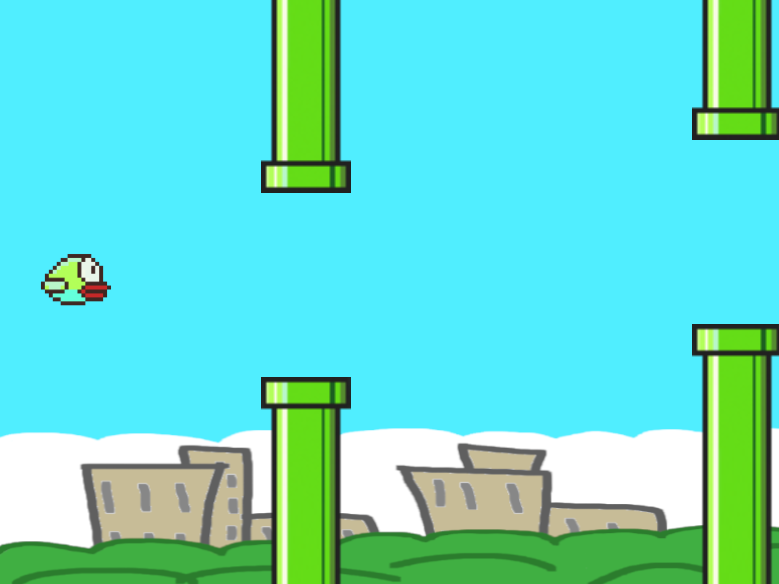
\includegraphics[scale=0.3]{images/game.png}
    \caption{Hra}
\end{figure*}

\subsection{Překážeky}
Z důvodu, že mi nepřišlo praktické pořád generovat nové překážky, tak jsem se rozhodl, že vytvořím celkem dvě dvojice překážek a ve chvíli, kdy překážka dojede mimo obrazovku, tak ji přesunu zpět na začátek a náhodně změním její výšku. A takto jsem se vyhl zbytečnému vytváření a ničení objektů. 

Pohyb překážek se postupně s rostoucím skóre zvyšuje.

\subsection{Hra počítačem}
Při vytváření programu, který za Vás hraje jsem musel dodržet podmínku, že počítač bude mít stejné podmínky jako skutečný hráč. To znamená, že počítač dostane jen souřadnice své polohy a souřadnice překážky, která následuje. Algoritmus na řešení tohoto problém spočívá v tom, že program zkontroluje zda je pták pod urovní překážky a pokud ano, tak zavolá metodu na vyskočení(která funguje stejně jako když hráč zmáčkne levé tlačítko myši), ale pokud je pták nad překážkou nechá ho dále padat.

\begin{figure*}[ht!]
    \centering
    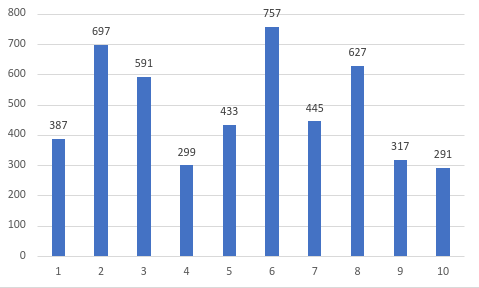
\includegraphics[scale=0.7]{images/graph.png}
    \caption{Graf skóre počítače}
\end{figure*}

